\documentclass[a4paper, 12pt]{article}
\usepackage[UTF8]{ctex}
% \usepackage[T1]{fontenc}
% \usepackage{inconsolata}


\usepackage{amsmath}
\usepackage{enumitem}
\setlist{
    nolistsep, % 去掉 item 和正文之间的间隔
    % labelindent=\parindent,
    leftmargin=*, % 保证小节标签缩进和上面对齐
    % labelsep=1em, % 标签后的空白
    align=left, % 标签对齐段落左边缘
}
\usepackage{tabularx}

\usepackage{graphicx}

\usepackage{geometry}
\geometry{
    a4paper,
    left=2cm,
    right=2cm,
    top=2cm,
    bottom=2cm,
}

\newcommand{\fs}[1]{\fontsize{#1 pt}{0pt}\selectfont}

\usepackage{mathtools}
\DeclarePairedDelimiter{\ceil}{\lceil}{\rceil}
\DeclarePairedDelimiter\floor{\lfloor}{\rfloor}

\usepackage{setspace}
% \setlength\parindent{0pt}
\setlength{\parindent}{2em} % 中文

% \newfontfamily\csl{Consolas}

\usepackage{array}
\newcolumntype{T}{>{\ttfamily}l}
\newcolumntype{Y}{>{\footnotesize\ttfamily}l}
\newcolumntype{y}{>{\footnotesize\ttfamily}c}

\usepackage{longtable}

\newcommand*{\thead}[1]{\multicolumn{1}{c}{\bfseries #1}}
\newcommand*{\yhead}[1]{\multicolumn{1}{c}{\footnotesize\bfseries #1}}

\newcommand{\ssa}{\phantom{x}}
\newcommand{\ssb}{\phantom{xx}}
\newcommand{\ssc}{\phantom{xxx}}
\newcommand{\ssd}{\phantom{xxxx}}
\newcommand{\sse}{\phantom{xxxxx}}

\usepackage{xcolor}
\usepackage{listings}
\definecolor{mygreen}{RGB}{28,172,0} % color values Red, Green, Blue
\definecolor{mylilas}{RGB}{170,55,241}

\newcommand{\ttf}{\ttfamily}

\lstdefinestyle{plainText}{language={},
    % basicstyle=\footnotesize \ttfamily,        % set font type and size
    basicstyle=\ttfamily,        % set font type and size
    breaklines=true,
    keywordstyle=\color{blue},
    % morekeywords={matlab2tikz},
    % morekeywords=[2]{1}, 
    % keywordstyle=[2]{\color{black}},
    identifierstyle=\color{black},
    stringstyle=\color{mylilas},
    % stringstyle=\color{purple},
    frame=single,
    framexleftmargin=0em,
    aboveskip=-\baselineskip,
    commentstyle=\color{mygreen},
    showstringspaces=false,% without this there will be a symbol in the places where there is a space
    % numbers=left,
    numbers=none,
    numberstyle={\tiny \color{black}}, % size of the numbers
    numbersep=9pt, % this defines how far the numbers are from the text
    tabsize=4,                     % sets default tabsize to 4 spaces
    emph=[1]{},
    emphstyle=[1]\color{red}, %some words to emphasise
    %emph=[2]{word1,word2}, 
    % emphstyle=[2]{style}, 
    escapeinside=``,               % Characters escape: To Use Chinese in codes   
}

\lstdefinestyle{myC}{language={C},
    % basicstyle=\footnotesize \ttfamily,        % set font type and size
    basicstyle=\ttfamily,        % set font type and size
    breaklines=true,
    keywordstyle=\color{blue},
    % morekeywords={matlab2tikz},
    % morekeywords=[2]{1}, 
    % keywordstyle=[2]{\color{black}},
    identifierstyle=\color{black},
    stringstyle=\color{mylilas},
    % stringstyle=\color{purple},
    frame=single,
    framexleftmargin=0em,
    aboveskip=-\baselineskip,
    commentstyle=\color{mygreen},
    showstringspaces=false,% without this there will be a symbol in the places where there is a space
    % numbers=left,
    numbers=left,
    numberstyle={\tiny \color{black}}, % size of the numbers
    numbersep=9pt, % this defines how far the numbers are from the text
    tabsize=4,                     % sets default tabsize to 4 spaces
    emph=[1]{printf},
    emphstyle=[1]\color{blue}, %some words to emphasise
    %emph=[2]{word1,word2}, 
    % emphstyle=[2]{style}, 
    escapeinside=``,               % Characters escape: To Use Chinese in codes   
}

\begin{document}

\begin{center}
{\fs{15}\bfseries {计算机动画原理与技术 ~大作业 ~报告}}

\vspace{0.5\baselineskip}

{\fs{15}\bfseries {Music-Driven Animation:音乐驱动式动画}}

\vspace{0.5\baselineskip}

{\fs{14} \kaishu 于泽汉 \hspace{1em} \textsf{No.118039910141}}
\end{center}

\section{答辩记录}

\subsection{音符的生成方式是什么?}
半随机生成。

每隔一段时间,在指定频率范围内(人耳可识别)随机生成一个基频,然后在这个基频的基础上再公式化生成其他频率。

支持同一时间多个频率,每个频率的持续时长也可不同。


\subsection{为什么要在基频的基础上生成其他频率?}
因为随机的几个频率同时发出,一般会令人产生“不安”的感觉。

为了提升演示效果,需要使这几个音在被人耳听到时显得更“和谐”一些。

从乐理上讲,这几个频率之间满足频率比尽可能接近较小的整数之比,比如 4:5:6 (大三和弦)就要比 160:192:231 (减三和弦)听起来更加和谐。

\subsection{用什么形式可视化这些音符?}

用空间上的二维扫描条形图的形式展示音符在时间上的持续和变化。

用颜色和纵轴位置来表征频率的高低。颜色上采用 HSL(色相、饱和度、明度)空间;纵轴上方是低频,下方是高频。

本来是打算纵坐标低的是低频、纵坐标高的是高频,这样符合直观。但是由于人眼习惯于注意正中偏上的区域,而低频部分通常音符较多,因此才采用现在的纵轴排布方案。

\subsection{说说用到的关键帧算法?}

这里其实用到的是比较简单的线性插值。

根据前后音符的频率和位置,线性插值出中间没有音符的那部分内容,从而将离散的音乐信号转换成连续的二维动画。

音符序列是事先生成好的,但其实一开始不生成所有音符也可以,只需要在插值时知道前后的音符频率即可。

关键帧是实时计算出来的。

对于前后音符数目不同的情况,也实现了保证视觉连续性的处理算法。

\subsection{有考虑过用一段音乐作为输入吗?}

考虑过。

但是因为普通的音乐文件混杂的其他信号太多,信噪比远不如自己生成的音符,因此要从中提取出重要的频率比较困难,工作量也很大。

实际上,从一段给定音乐中提取出每个时刻主导性的基音和泛音也是一个比较热门的研究课题。

因此为了使演示效果更好,降低实现的复杂度,最终采用了更加简洁抽象的随机生成音符。

\subsection{进一步的改进计划?}

目前音符的生成还比较简单,之后可能会加入更丰富的生成模式。

目前用的最简单的线性插值算法,之后可能会采用更柔和或者是自适应的插值方式,改进关键帧的连续性和流畅度。

目前的可视化形式还比较朴素,之后也许会加入其它元素。


\section{问题概述}

\subsection{背景}
当前,对各种信息和数据进行可视化的研究工作层出不穷,但是对声音的可视化大多停留在离散的频谱和振幅直方图的朴素形式,只有少部分会依据时间上前后的序列,产生中间的关键帧,以提高可视化的连续性和流畅度。

\subsection{动机和意义}

一方面是探索前沿的音乐可视化形式,另一方面是为了将音频和动画整合起来,实现这样一个完整的流水线。

\section{相关工作}

\subsection{Inverse-Foley Animation}

这个工作基于声音信号,仿真出相应的物理运动动画。下图展示了这一工作的具体流程:

\begin{center}
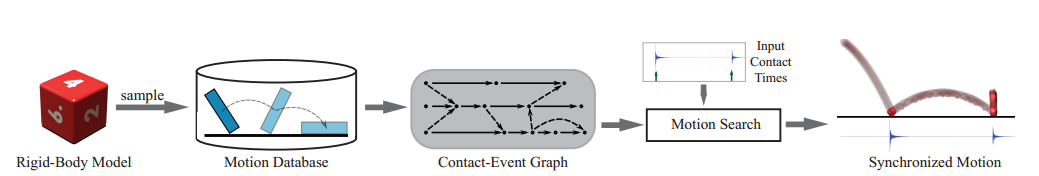
\includegraphics[width=\textwidth]{images/inverse_foley.png}\\
Inverse-Foley 的实现流程
\end{center}

这个工作分为如下几个步骤:

1. 建立刚体模型

2. 使用刚体模型生成运动数据集

3. 根据这些运动数据集建立联系-事件图

4. 根据输入声音信号搜索运动路径

5. 仿真运动动画,使之与声音信号同步


\subsection{Data-driven Autocompletion for Keyframe Animation}

这个工作基于给定的关键帧,自动补全其他部分动画。

具体工作见下列各图说明:

\begin{center}
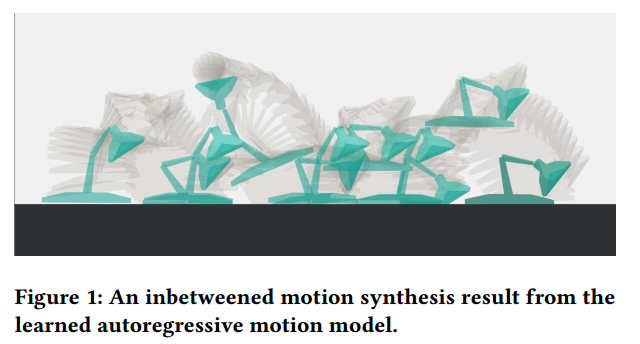
\includegraphics[width=0.8\textwidth]{images/fig1.png}\\
绿色部分表示给定的关键帧,灰色部分表示补全出来的动画
\end{center}


\begin{center}
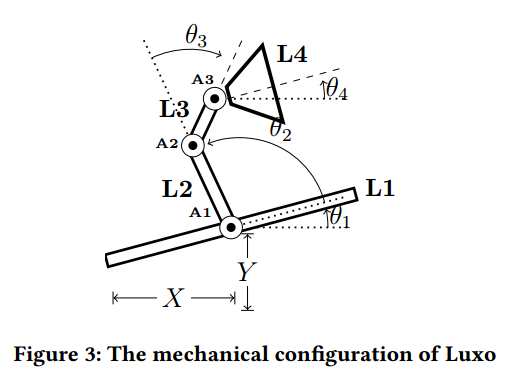
\includegraphics[width=0.8\textwidth]{images/fig3.png}\\
本文作者自己建立的刚体模型,用于生成训练集
\end{center}

\begin{center}
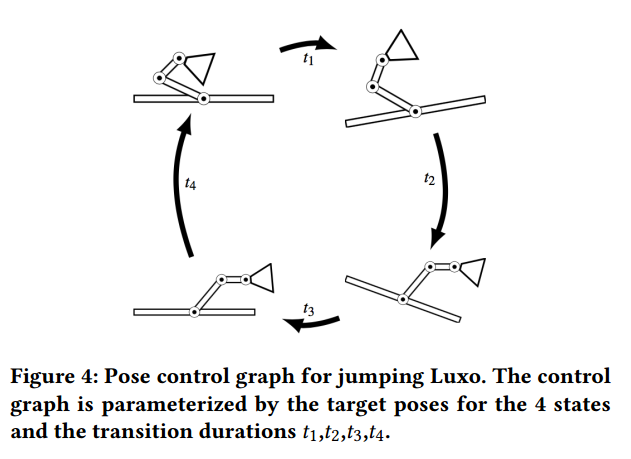
\includegraphics[width=0.8\textwidth]{images/fig4.png}\\
该刚体的动力学模型和状态机
\end{center}

\begin{center}
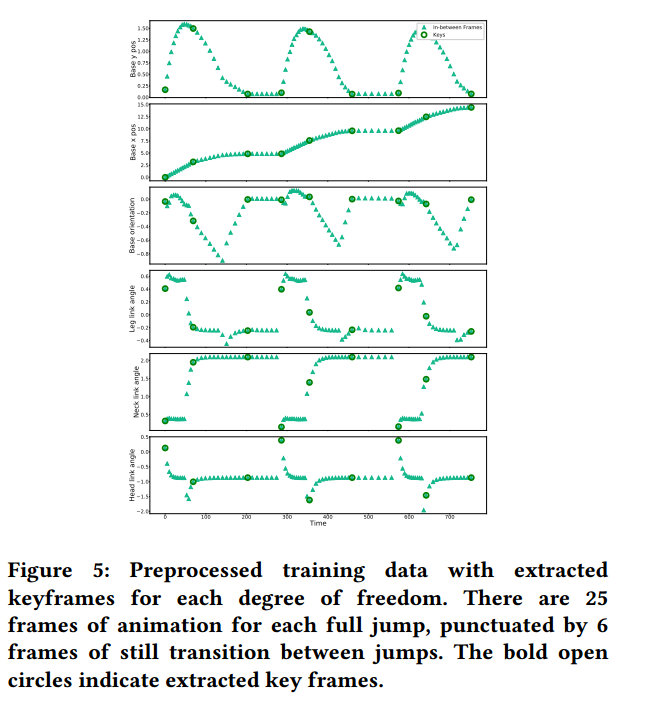
\includegraphics[width=0.8\textwidth]{images/fig5.png}\\
对该刚体模型的运动进行训练,并采集训练数据
\end{center}

\begin{center}
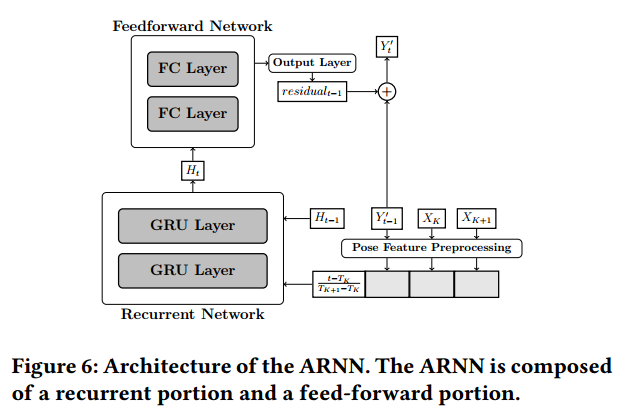
\includegraphics[width=0.8\textwidth]{images/fig6.png}\\
本文采用的 ARNN 机器学习训练框架
\end{center}

\section{实验目标}

用音乐驱动动画:

1. 输入:音乐信号的数字化表示

2. 处理:将这些\textbf{离散的声音信号}转换成\textbf{连续的二维动画}

3. 输出:二维连续动画


\section{实验技术}

\subsection{音符的半随机生成}

\begin{itemize}[leftmargin=*]
\item 随机生成的音符听感很差:
    \begin{itemize}[leftmargin=*]
    \item 随机音符组合的声音不够和谐
    \end{itemize}
\item 确保音符组合听起来较为和谐:
    \begin{itemize}[leftmargin=*]
    \item 保证同一时间演奏的音符尽可能接近和弦
    \item 频率比尽可能接近较小的整数比
    \end{itemize}
\item 多种生成模式:
    \begin{itemize}[leftmargin=*]
    \item 同一时刻可以生成多个通道
    \item 不同时刻的音符持续时长不同
    \end{itemize}
\end{itemize}

\subsection{音符可视化}

\begin{itemize}[leftmargin=*]
\item 用颜色和相对位置来区别频率:
    \begin{itemize}[leftmargin=*]
    \item HSL(色相、饱和度、明度)色彩空间
    \item 纵轴高度和频率相关
    \end{itemize}
\item 空间上的条形图展示音乐的时间维度:

\item 两种刷新缓存的模式:
    \begin{itemize}[leftmargin=*]
    \item 保证绘制精确度:经常更新的区域每帧刷新
    \item 提高绘制效率:不常更新或局部更新的区域保留之前的帧
    \end{itemize}
\end{itemize}

\begin{center}
\includegraphics[width=0.7\textwidth]{images/update_regions.png}\\
红色框内的区域每帧全部更新,黄色框内的区域只更新新绘制的部分
\end{center}

\subsection{插值与关键帧}

\begin{itemize}[leftmargin=*]
\item 将离散的信号插值成连续的动画:
    \begin{itemize}[leftmargin=*]
    \item 线性插值(更柔和的S型插值)
    \item 预先生成音符序列
    \item 实时计算关键帧
    \end{itemize}
\end{itemize}

\begin{center}
\includegraphics[width=0.9\textwidth]{images/keyframe.png}\\
左边是没有加入关键帧的可视化效果,右边是线性插值后的效果
\end{center}

\subsection{视觉连续性处理算法}

\begin{itemize}[leftmargin=*]
\item 保持视觉上的连续性
    \begin{itemize}[leftmargin=*]
    \item 每条通道和前后通道都有连接
    \item 连接尽可能均匀分布
    \end{itemize}
\end{itemize}

\begin{center}
\includegraphics[width=0.3\textwidth]{images/continue.png}\\
前后时刻通道数有可能不同:蓝色,前少后多;红色,前后相同;黄色,前多后少

\end{center}

\section{结果展示}

\begin{center}
\includegraphics[width=0.9\textwidth]{images/result_preview_withoutkey_x.png}\\
没有加入关键帧的离散可视化效果
\end{center}

\begin{center}
\includegraphics[width=0.9\textwidth]{images/result_preview_x.png}\\
加入关键帧后的连续可视化效果
\end{center}

\newpage

\section{总结与改进}

\subsection{实验总结}

\begin{itemize}[leftmargin=*]
\item 实现了较好的音符生成算法
\item 实现了离散音乐信号的实时连续动画化
\item 实现了插值算法和关键帧技术
\item 完成了若干细节上的优化
\end{itemize}

\subsection{进一步工作}

目前音符的生成还比较简单,之后可能会加入更丰富的生成模式。

目前用的最简单的线性插值算法,之后可能会采用更柔和或者是自适应的插值方式,改进关键帧的连续性和流畅度。

目前的可视化形式还比较朴素,之后也许会加入其它更加新颖的元素。

\section{参考文献}

1. Inverse-Foley Animation: Synchronizing rigid-body motions to sound

2. Automatic Synchronization of Background Music and Motion in Computer Animation

3. Plausible motion simulation for computer graphics animation

4. Interactive Spacetime Control for Animation

5. Synthesizing Sounds from Physically Based Motion

6. Evaluating the visual fidelity of physically based animations

7. Interactive manipulation of rigid body simulations

8. Computer Puppetry: An Importance-Based Approach

9. Physically-based sound effects for interactive simulation and animation


\end{document}